\documentclass{article}
% \usepackage{showframe}
\usepackage{siunitx}
\usepackage{booktabs}
\usepackage{graphicx}
\usepackage{amsmath}
\usepackage{mathtools}
\usepackage{minted}
\usepackage{tabularx}
\usepackage{url}
% \usepackage{subfig}
\usemintedstyle{xcode}

% \usepackage{fullpage}

\frenchspacing
% \setlength{\parindent}{0ex}
% \setlength{\parskip}{3 ex plus 2 ex minus 1 ex}

\title{Homework 6}
\author{Josh Bradt}
\date{February 29, 2016}

\begin{document}

\maketitle

I modified the code from the second homework assignment such that the loop being timed was this:
\begin{minted}[gobble=4]{C}
    for (size_t iter = 0; iter < numIters; iter++) {
    #pragma omp parallel for default(none) shared(c,a,N) schedule(static)
        for (size_t i = 0; i < N; i++) {
            c[i] = a[i];
        }
        dummy(a, c);
    }
\end{minted}
I compiled the code using the Intel compiler with no optimization. (I had to do this since the optimizer was replacing the element-by-element copy with a single call to an optimized version of \texttt{memcpy}.) I then ran it for an array size of $N=\num{50000000}$ with 20 iterations. For comparison, I ran the code both on my quad-core Mac Mini and on the HPCC's \texttt{dev-intel14} node, which has two 10-core processors. The results are listed in Table~\ref{tab:results} and plotted in Figure~\ref{fig:plots}.

In both cases, the performance seems to increase nearly linearly until the number of threads approaches the number of physical cores in the system.\footnote{Though in the case of the HPCC, this limit is instead at the number of cores in \emph{one} of the two processors. This may reflect limitations of memory sharing between the two processors, or it may indicate that all of the threads were scheduled on one processor each time.} After that, the performance levels off. This matches well with the suggested model of $R = \min(N_t R_1, R_\text{max})$, where $N_t$ is the number of threads and $R_1$ and $R_\text{max}$ are the rate with one thread and the maximum observed rate, respectively.

\begin{table}[p]
\centering
\begin{tabular}{S[table-format=2]
                S[table-format=1.4]
                S[table-format=5]
                S[table-format=1.4]
                S[table-format=5]}
\toprule
{Num Threads} & {Mac Time} & {Mac Rate} & {HPCC Time} & {HPCC Rate} \\
{} & {[s]} & {[MB/s]} & {[s]} & {[MB/s]} \\
\midrule
1           & 0.1400   & 5730     & 0.1700    & 4700      \\
2           & 0.0763   & 10500    & 0.0816    & 9810      \\
4           & 0.0656   & 12200    & 0.0424    & 18800     \\
6           & 0.0659   & 12100    & 0.0284    & 28200     \\
8           & 0.0660   & 12100    & 0.0221    & 36300     \\
10          & 0.0653   & 12200    & 0.0187    & 42900     \\
12          & 0.0654   & 12200    & 0.0175    & 45700     \\
14          & 0.0657   & 12200    & 0.0164    & 48600     \\
16          & 0.0657   & 12200    & 0.0184    & 43400     \\ \bottomrule
\end{tabular}
\caption{Result of the measurement on both a quad-core Mac desktop and the 2~$\times$~10-core \texttt{dev-intel14} node.}
\label{tab:results}
\end{table}

\begin{figure}[p]
    \centering
    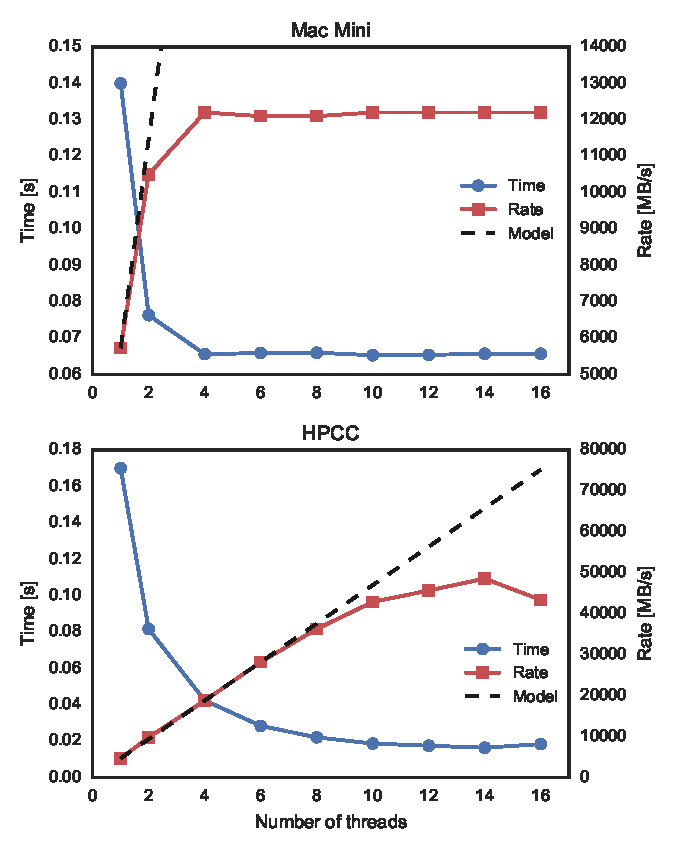
\includegraphics{plots.pdf}
    \caption{The results of running on the two computers. In each case, the performance levels off around when the number of threads equals the number of physical cores in one processor (4 for the Mac Mini, and 10 for the HPCC). The models shown are $R=N_t R_1$ where $N_t$ is the number of threads and $R_1$ is the rate for one thread.}
    \label{fig:plots}
\end{figure}

\end{document}
